\documentclass[baaa]{baaa}
\usepackage{ragged2e} 
\usepackage[pdftex]{hyperref}
\usepackage{subfigure}
\usepackage{natbib}
\usepackage{booktabs}
\usepackage{amsmath}
\usepackage{helvet,soul}
\usepackage[font=small]{caption}
\usepackage{siunitx}
\usepackage[normalem]{ulem}

\useunder{\uline}{\ul}{}
\contriblanguage{1}

\contribtype{1}
\thematicarea{99}
\received{\ldots}
\accepted{\ldots}

%%%%%%%%%%%%%%%%%%%%%%%%%%%%%%%%%%%%%%%%%%%%%%%%%%%%%%%%%%%%%%%%%%%%%%%%%%%%%%
\title{Generadores de números aleatorios con Python}
\titlerunning{Generadores de números aleatorios}

\author{J. M. Puddu \inst{1}}

\authorrunning{J. M. Puddu }

\contact{julieta.puddu@mi.unc.edu.ar}

\institute{
Facultad de Matemática, Astronomía, Física y Computación, UNC, Argentina
}

\resumen{Este trabajo presenta una implementación computacional de métodos estadísticos para la generación, validación y análisis de distribuciones de probabilidad. Se estudiaron distribuciones tanto continuas (Fisher-Tippett, Normal) como discretas (Poisson, Binomial), aplicando el método de la transformada inversa para generar variables aleatorias que sigan estas distribuciones. La técnica de bootstrap fue empleada para estimar parámetros poblacionales a partir de muestras, demostrando su efectividad en la recuperación de valores teóricos como la media ($E(F) = 0.57721\sigma$ para Fisher-Tippett) y varianza. La validación estadística se realizó mediante el test $\chi^2$ de Pearson, que permitió verificar la bondad de un ajuste, obteniendo p-valores de 0.98 para datos binomiales y identificando correctamente muestras no pertenecientes a la distribución teórica. Como aplicación práctica, se implementó el experimento de Buffon para la estimación de $\pi$, alcanzando una precisión de $\pm0.08$ con 10,000 replicaciones.}

\keywords{https://github.com/shulypuddu/astrometria/tree/main}
\begin{document}
\maketitle

\section{Introducción}
Este trabajo se centra en las distribuciones de probabilidad, tanto continuas como discretas y en como podemos trabajar con variables aleatorias que sigan una dada distribución. Por tanto, y a modo de introducción, se definen las distribuciones con las que se trabajó:

\subsection{Distribución de Fisher-Tippett}
 
Es una distribución continua desarrollada por R.A. Fisher y L.H.C. Tippett  también conocida como distribución GEV (\textit{Generalized Extreme Value}) ya que su definición nace de generalizar 3 familias de funciones distintas. 


La distribución se define como:
\begin{equation}
    f(x,\mu,\sigma,\xi)= \frac{1}{\sigma}t(x)^{\xi+1}e^{t(x)}
\end{equation}
donde la función $t(x)$ se define según el valor de $\xi$ como:
\begin{equation}
 t(x) = 
 \begin{cases}
 \left(1+\xi\dfrac{x-\mu}{\sigma}\right)^{-1/\xi} & \text{para } \xi \neq 0 \\[8pt]
 e^{-(x-\mu)/\sigma} & \text{para } \xi = 0
 \end{cases}
\end{equation} 
Esta lleva 3 parámetros que la caracterizan:
\begin{itemize}
    \item \textbf{Parámetro de la forma $\xi$: }dependiendo si $\xi=0$, $\xi>0$, ó $\xi<0$ la distribución va a ser igual a la de  Gumbel, Fréchet ó Weibull respectivamente. 
    \item \textbf{Parámetro de locación $\mu$: }indica donde se centra el pico de la distribución.
    \item \textbf{Parámetro de escala $\sigma$: }indica la dispersión de la función.
\end{itemize}
Una característica de interés es que si elegimos $\mu=0$ y $\xi=0$ entonces el valor de expectación de la distribución se reduce a $E(F)=0.57721\sigma$

\subsection{Distribución Normal o Gaussiana}
Probablemente la más conocida de todas las mencionadas en este trabajo. Una variable aleatoria continua  $X$  se dice normalmente distribuida con media $\mu$  y varianza $\sigma^2$  si su función de densidad de probabilidad está dada por

\begin{equation}
f_X(x) = \frac{1}{\sqrt{2\pi}\sigma} e^{-\frac{(x - \mu)^2}{2\sigma^2}} 
\end{equation}
Cabe destacar que $\mu$ es tanto el parámetro de locación como la media de la distribución, al igual que $\sigma$ es el parámetro de dispersión y se relaciona directamente con la varianza.

\subsection{Distribución de Poisson}
Es una distribución discreta por lo que los valores de entrada son números enteros, estas distribuciones responden a aquellos experimentos donde 
con el modelo de Poisson se determina la probabilidad de ocurrencia de un determinado evento en el tiempo o el espacio y no en un número definido de repeticiones del experimento. En estos eventos que se producen aleatoriamente en el espacio o el tiempo, la frecuencia de ocurrencia de un evento es tan baja con relación a la frecuencia de no ocurrencia que se consideran como sucesos raros. Tratar de describir la distribución de una variable aleatoria de este tipo mediante el modelo binomial sería impráctico puesto que el número de ensayos tendría que ser extraordinariamente grande para que ocurriera el resultado esperado.

Luego, la función de probabilidades para el modelo de Poisson queda:

\begin{equation}
    P(x=i)= \frac{e^{- \lambda}}{i!}\lambda ^i 
\end{equation}

con $\lambda$ el número promedio de ocurrencias en un espacio o tiempo dado y k el número de veces que ocurre el éxito en ese mismo espacio o tiempo.


Esta distribución cumple que tanto la media como la varianza son iguales al parámetro $\lambda$.

\subsection{Distribución binomial}
Al igual que la distribución de Poisson es una distribución discreta, en este caso, esta distribución responde a aquellos experimentos que tienen solamente 2 resultados (de ahí el nombre) es decir cualquier experimento que podamos obtener ``éxito" o ``fracaso". Esta distribución se define como: 
\begin{equation}
    B(x=i)= \binom{n}{i}p^i(1-p)^{n-i}
\end{equation}
Donde $\binom{n}{i}$ es el número combinatorio.

Esta distribución cumple que las siguientes relaciones para la media ($E$) y la varianza ($Var$)
\[E(X) = np \quad Var(X) = np(1 - p)\]

\section{Método de la transformada inversa}
Este es un método para generar variables aleatorias que sigan una dada distribución.
Aprovechando que la función de distribución acumulada (CDF) es una función creciente y que esta limitada dentro del intervalo $(0,1)$ buscamos su función inversa y generamos un conjunto de números aleatorios y al evaluarlos en la función inversa obtenemos un nuevo conjunto de números cuya distribución de frecuencias sigue a la PDF deseada.

\[
p(X) \to F(X) \to F^{-1}(U)=x \to f(x)==p(X)
\]

\subsection{Distribución de Fisher-Tippett}
Para aplicar este método a la distribución de Fisher-Tippett se trabajó con el caso particular de $\xi=0$ y $\mu=0$, donde la función inversa esta definida según la ecuación \ref{eq:f-1ft}
\begin{equation}
    F^{-1}(y)=-\sigma\:ln(\:ln(y)\:)
\label{eq:f-1ft}
\end{equation}
Tomando $\sigma=2$ obtenemos la distribución vista en la figura \ref{fig:ftanalisis}, la cual nos da un valor de expectación de $1.084747$, al reemplazar $\sigma$ 
\begin{figure}[h]
    \centering
    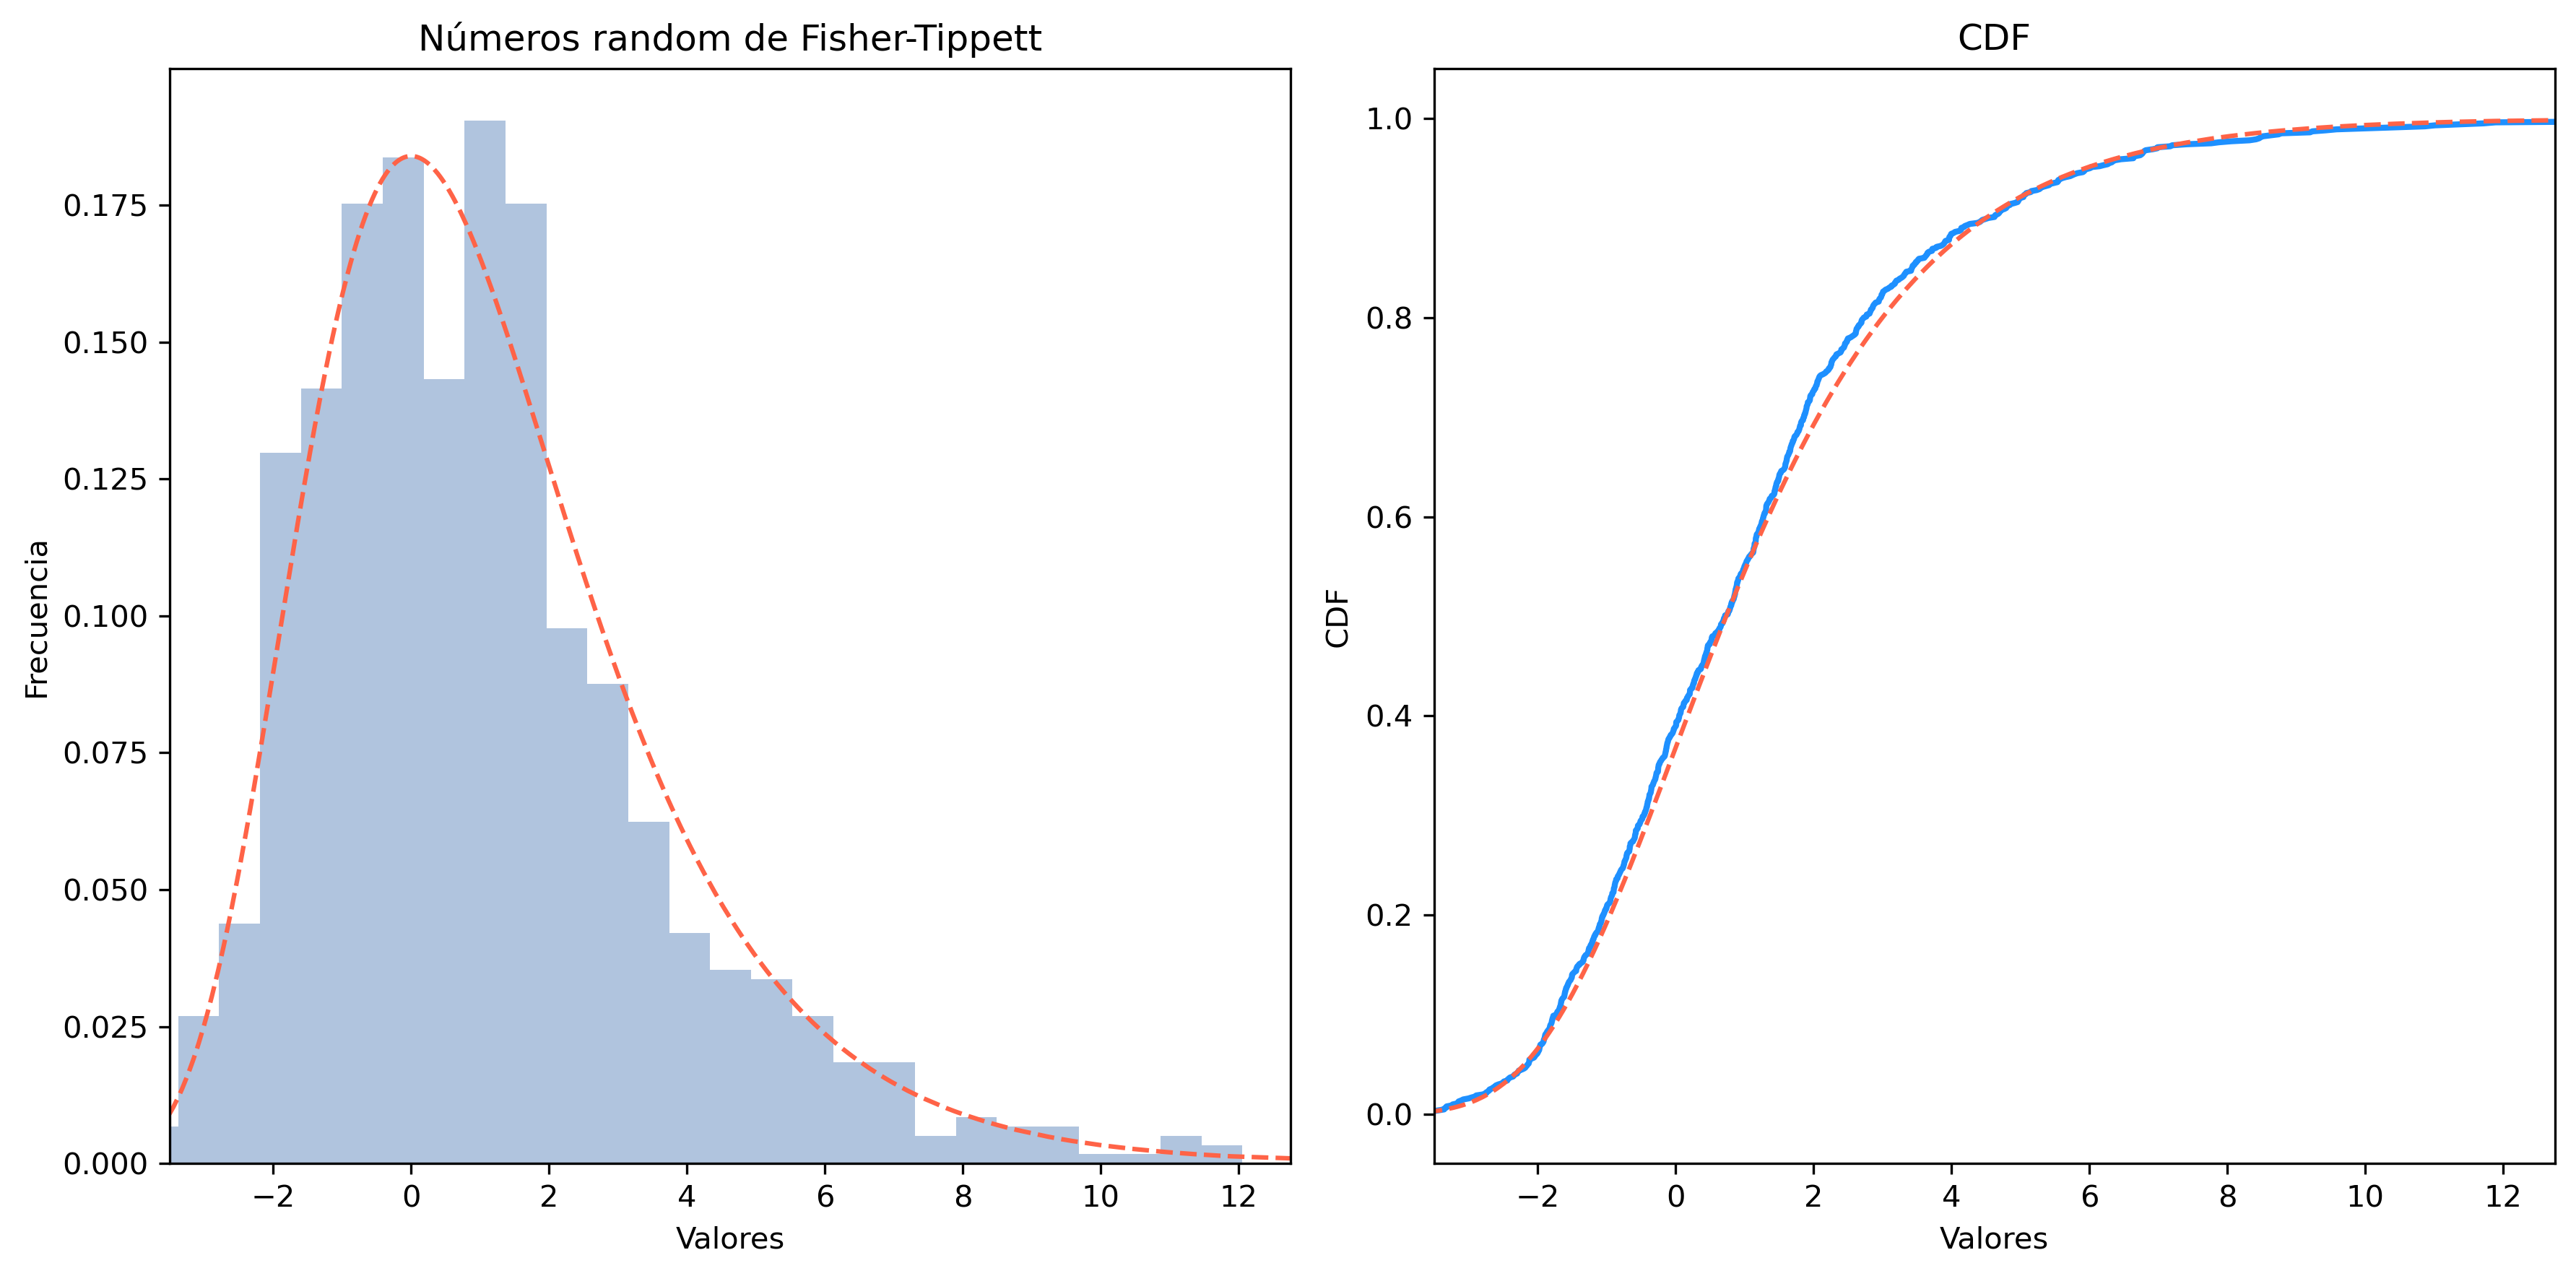
\includegraphics[width=\linewidth]{imagenes/ft_analysis.png}
    \caption{Distribución de frecuencia y frecuencia acumulada de una muestra aleatoria, superpuestas las respectivas distribuciones de Fisher-Tippett }
    \label{fig:ftanalisis}
\end{figure}

\subsection{Distribución de Poisson}
Para este caso, planteamos una cantidad de 5 eventos por hora y un tiempo de 3 hs.
Es decir, vamos a modelar una distribución de Poisson con $\lambda=5$ y esperamos ver que al llegar a las 3hs los datos generados tengan una media de 15 eventos.

La función inversa utilizada fue: \[F^{-1}(y)=1/\lambda\:ln(1-y) \] y con esta obtuvimos los ``caminos'' vistos en la figura \ref{fig:poisson}

\begin{figure}[h]
    \centering
    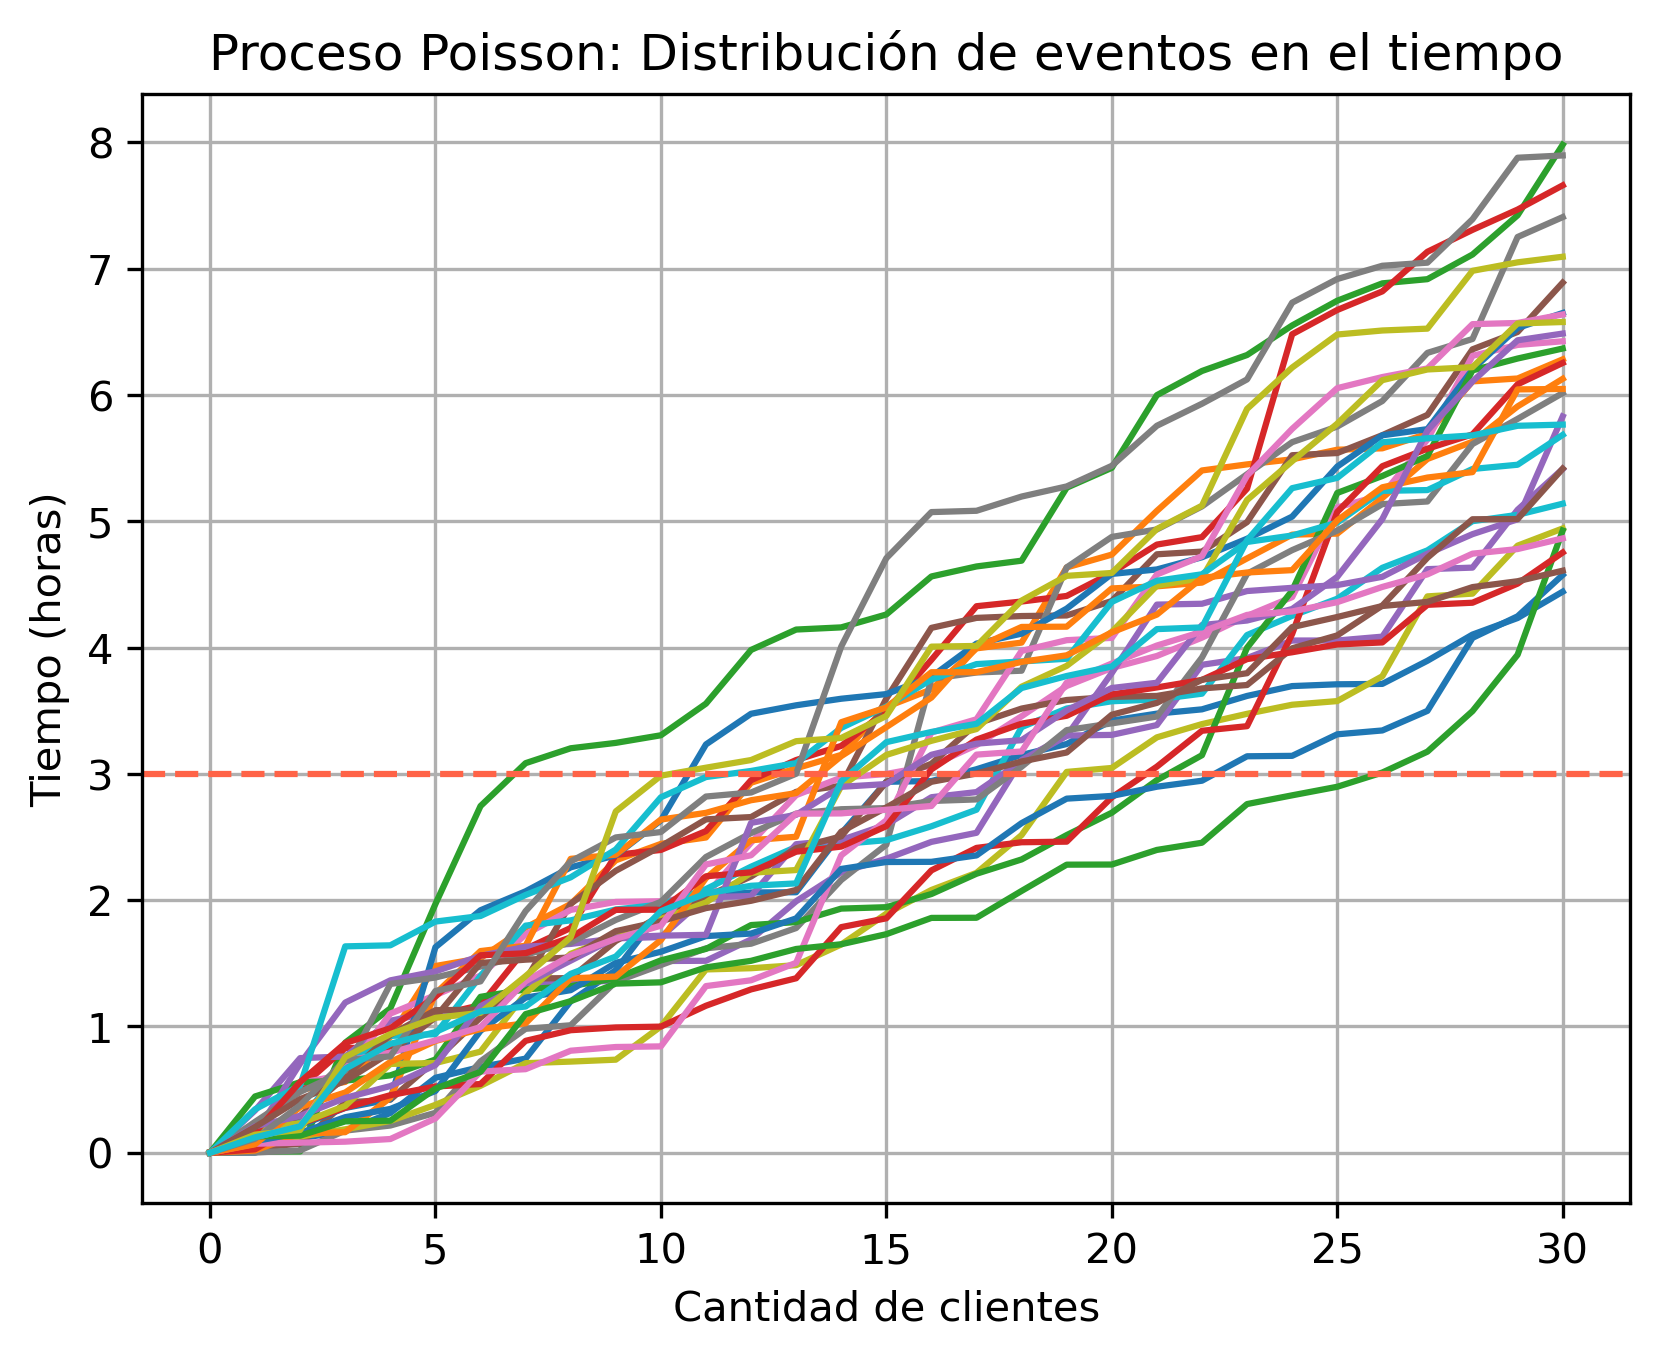
\includegraphics[width=\linewidth]{imagenes/poisson.png}
    \caption{Distribución de frecuencias de los eventos a lo largo del tiempo siguiendo distribuciones de Poisson}
    \label{fig:poisson}
\end{figure}
Ahora de estos solamente me interesa cuando el tiempo sean 3hs, para esto veo la cantidad de clientes en cada experimento a este tiempo y grafico un histograma con sus respectivas frecuencias, este debería seguir una distribución de Poisson con $\lambda=15$ (ya que estamos ``normalizando'' la unidad de tiempo). Esto es lo que muestra la figura \ref{fig:poisson3h} y efectivamente coincide con la distribución deseada.  
\begin{figure}[h]
    \centering
    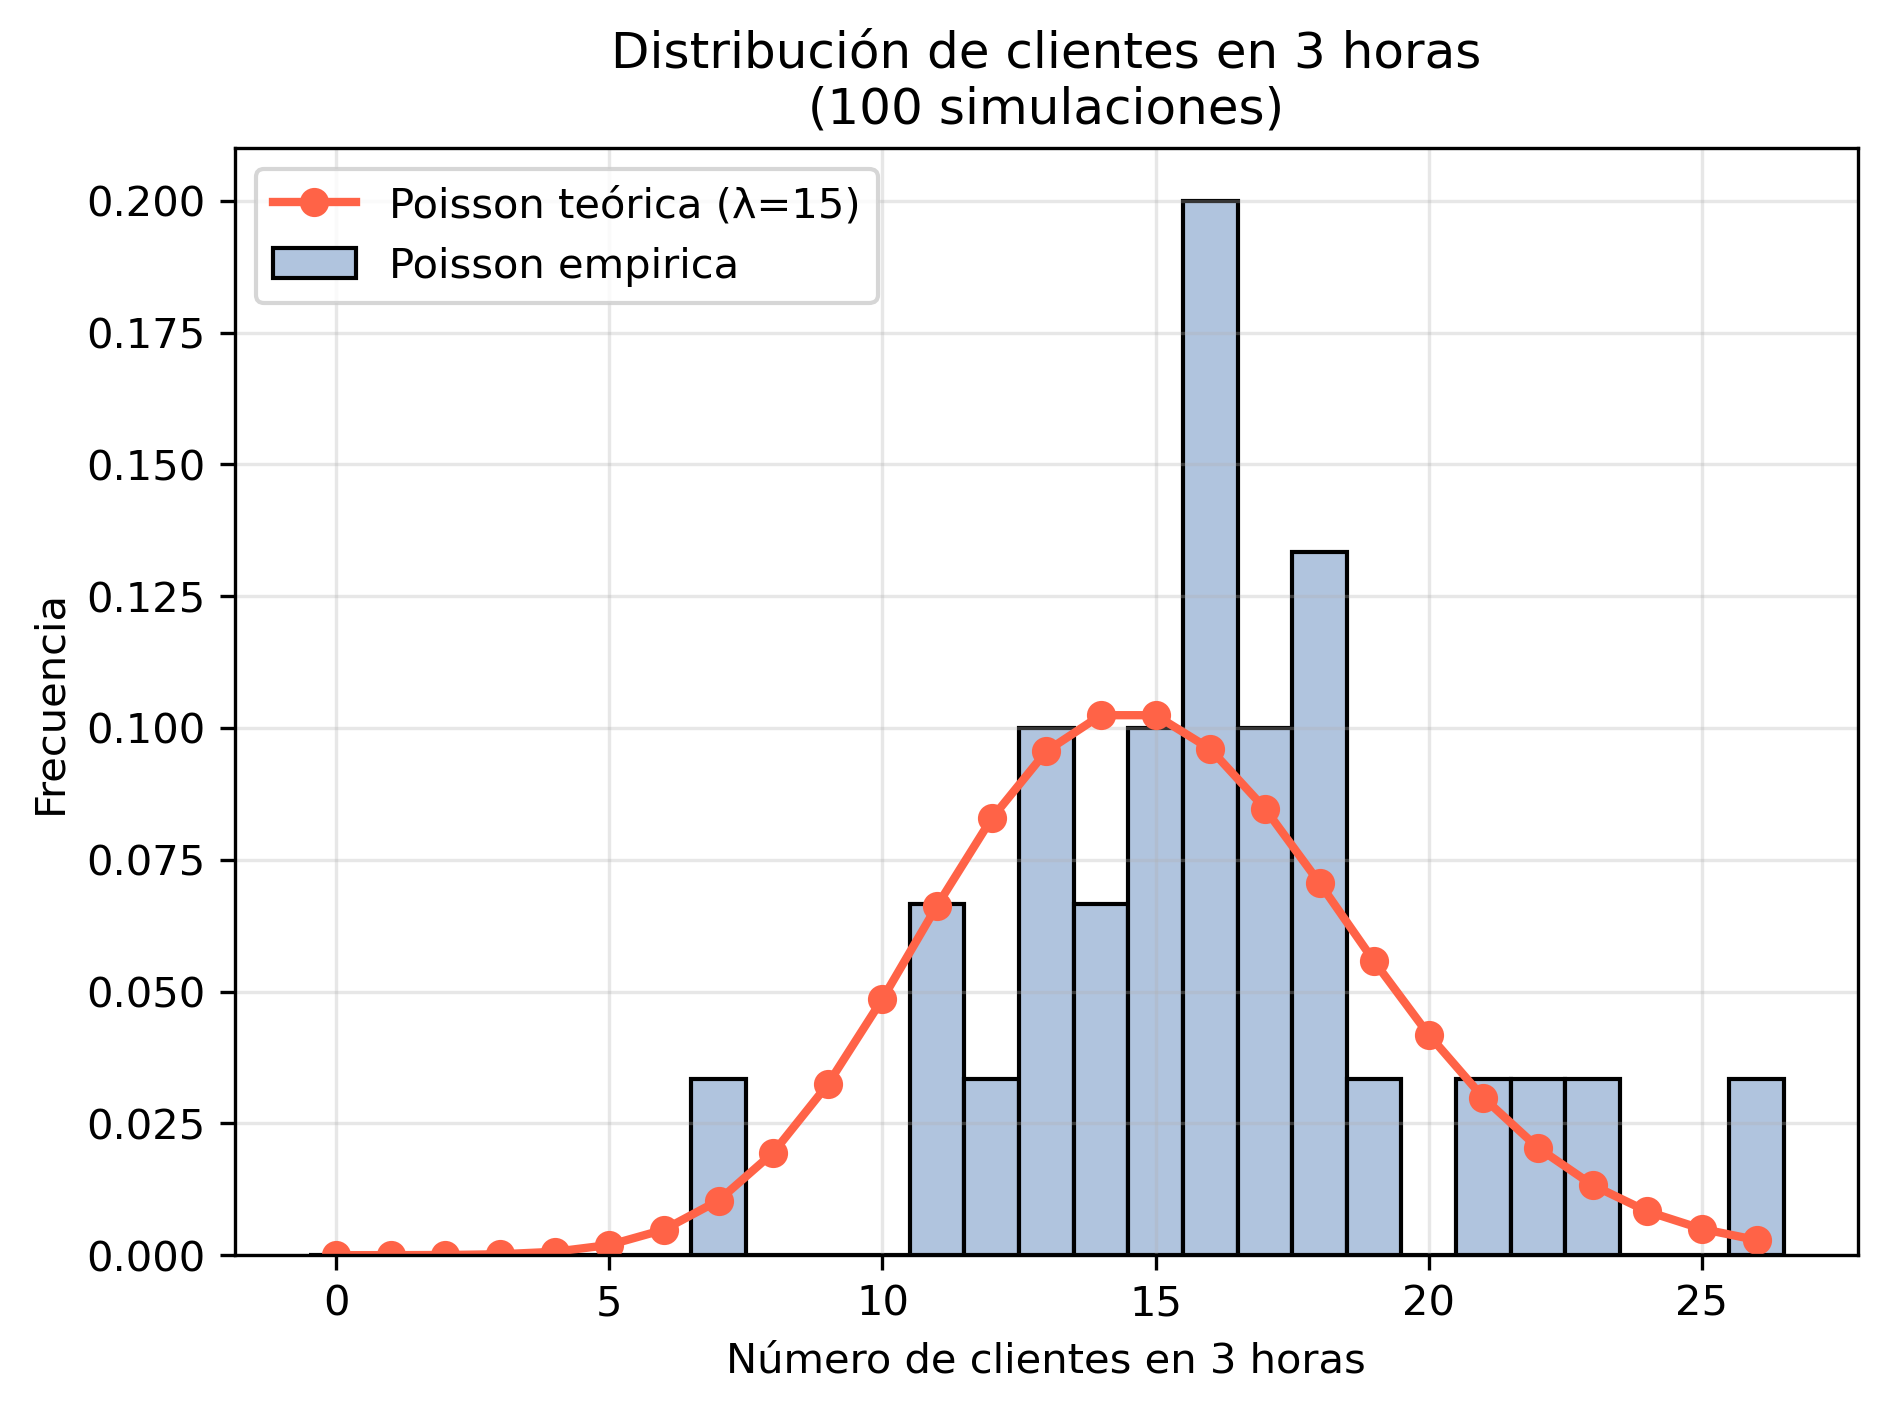
\includegraphics[width=\linewidth]{imagenes/poisson_completo.png}
    \caption{Distribución de frecuencia de eventos a las 3hs. Superpuesta la distribución de Poisson con $\lambda=15$ }
    \label{fig:poisson3h}
\end{figure}



\section{Técnica de bootstrap}
La técnica de bootstrap es aquella que recupera información a partir de los datos sin asumir ninguna hipótesis de estos. Para ello se crean \textit{muestras bootstrap}, las cuales son muestras aleatorias del conjunto de datos original y con el mismo tamaño que este. Dicho de otro modo, si se han obtenido $n$ observaciones $\{x_1,x_2,...,x_n\}$, una muestra bootstrap es una muestra aleatoria de tamaño $n$ tomada aleatoriamente de $\{x_1,x_2,...,x_n\}$ y permitiendo repeticiones.  

Esta técnica resulta útil para estimar valores o parámetros de la distribución de probabilidad del conjunto original sin necesidad que conocer dicha distribución a partir de una distribución empírica. 
Para probar este método se generaron 2 conjuntos datos, uno usando una distribución Gaussiana y otro usando una distribución de Fisher-Tippett y se uso la técnica de bootstrap para calcular el valor de expectación y la varianza de cada uno. 

\subsection{Datos generados con la distribución Gaussiana:} 
Usando las funciones de la librería \textit{SciPy}  se generaron 1000 valores siguiendo una distribución normal ccon parámetros $\mu=0$ y $\sigma=1$, se eligió esta distribución ya que se cumple que $E(F)=0$ y $Var(F)=\sigma$, por tanto se conocen los valores teóricos para comparar con los obtenidos por la técnica bootstrap.

Como resultado del re-muestreo se obtienen los diagramas mostrados en la figura \ref{fig:norm_boots}, como vemos logran repetir muy bien las valores originales del conjunto de datos y ademas los valores teóricos entran dentro de un intervalo de confianza de $95\%$

\begin{figure}[h]
    \centering
    
\includegraphics[width=\linewidth]{imagenes/bootstrap.png}
    \caption{Distribuciones de las media y varianza de las muestras bootstrap para una distribución normal.}
    \label{fig:norm_boots}
\end{figure}

\subsection{Datos generados con la distribución de Fisher-Tippett:} 
En este caso se uso un conjunto de 1000 datos generados con el método de la transformada inversa de modo que sigan a una distribución de Fisher-Tippett pero con parámetros ($\xi=0$,$\mu=0$,$\sigma=1$), donde el valor de expectación de la distribución es $0.57721$ y la varianza teórica $1.28255$ y del remuestreo obtenemos los diagramas que se muestran en la figura \ref{fig:ft_boots}, como vemos se repiten las mismas conclusiones que con la distribución normal.

\begin{figure}[h]
    \centering
    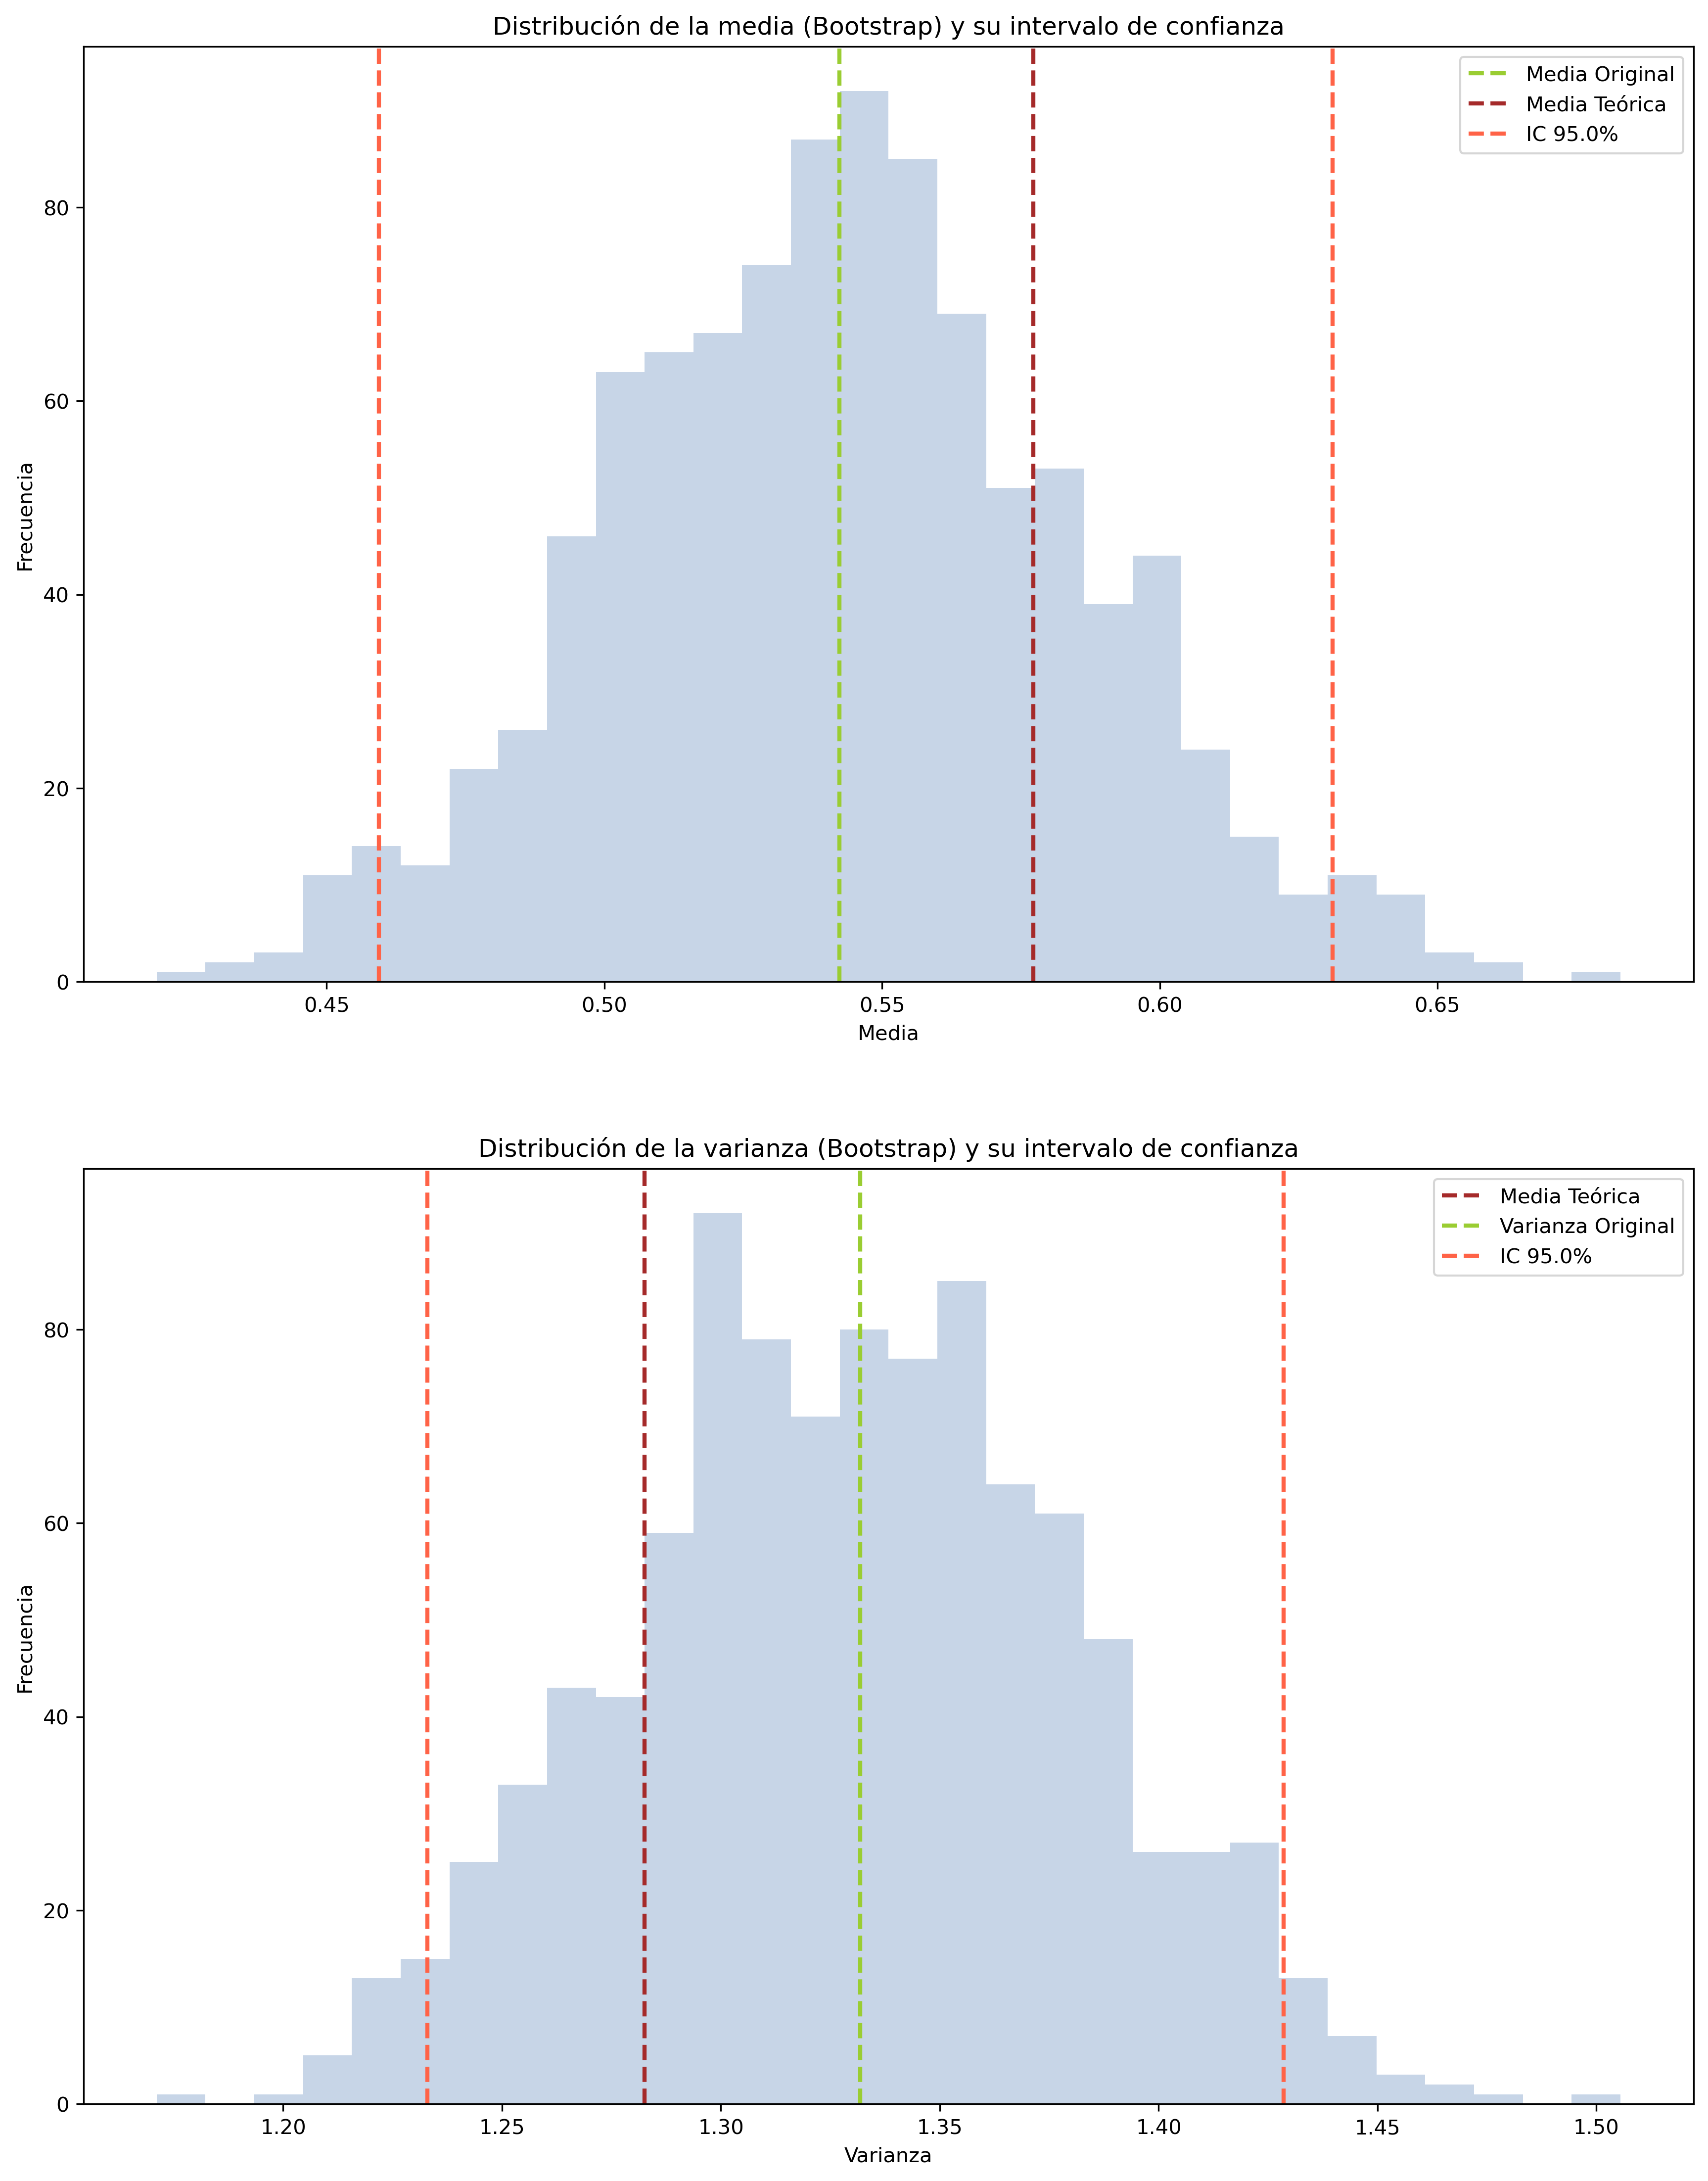
\includegraphics[width=\linewidth]{imagenes/ft_bootstrap.png}
    \caption{Distribuciones de las media y varianza de las muestras bootstrap para una distribución de Fisher-Tippett.}
    \label{fig:ft_boots}
\end{figure}


\section{Técnicas de validación estadística}
Una vez que ajustamos una cierta distribución a un conjunto de datos es importante saber que tan ``bueno'' fue ese ajuste, para esto se debe aplicar una técnica de validación estadística, en este trabajo se incluye el test de $\chi^2$ de Pearson.

\subsection{Test de chi-cuadrado}
En este caso definimos como estadístico de prueba a  

\[
T = \sum_{i=1}^{k} \frac{(N_i - n p_i)^2}{n p_i}
\]
Donde $p_i$ es la probabilidad que una variable con distribución $F$ tome el valor $i$, y $N_i$ es la frecuencia con la que el valor $i$ aparece en la muestra, es decir, la frecuencia observada.

Si el valor de $T$ es grande, se considera que hay evidencias que la muestra no proviene de la distribución $F$: se rechaza la hipótesis nula. Por el contrario, si el valor de $T$ es pequeño, no hay evidencias suficientes para rechazar la hipótesis. Si la hipótesis nula es cierta y $n$ es grande, entonces el estadístico $T$ tiene una distribución $\chi$-cuadrado con $k - 1$ grados de libertad: $\chi_{k-1}^2$.

Con esto definimos el \textit{valor-$p$}, el cual es quien nos dice si aceptamos o no una hipótesis, este se define según: $p = P_{H_0} (t \geq T) \leq  \alpha$, donde $t$ es el valor teórico que depende de la distribución del test que se use, en este caso $t=\chi^2_{k-1}$ y donde $\alpha$ nos dice el nivel de rechazo. Entonces si el nivel de rechazo es del $5\%$, entonces un $p$-valor menor que $0.05$ es indicativo que la muestra no proviene de la distribución $F$, es decir, que debe rechazarse la hipótesis nula. Por el contrario, valores de $p$ más grandes no dan evidencia que se deba rechazar la hipótesis.

Si en cambio se rechaza al $1\%$ entonces un \textit{valor-$p$} menor a $0.01$ indicará que se debe rechazar la hipótesis nula.

Para aplicar este test se uso como distribución teórica a una distribución binomial con parámetros $p=0.4$ y $n=10$, y se la comparo con datos producidos a partir de: 100 observaciones de una variable aleatoria producida usando el método de la transformada inversa con la misma distribución binomial y 100 observaciones de una V.A. que sigue una distribución normal con $\sigma=2.5$ y $2\leq\mu\leq7$ 
En todos los casos se trabajo con intervalos de confianza de $95\%$ y se uso la librería de \textit{SciPy} para obtener el $\chi_{critico}$, además en todos los casos se estableció como hipótesis nula $H_0$ \textit{``la muestra sigue una distribución binomial''} 

En el primer caso se obtuvo que $\chi^2=3.024$ y un \textit{valor-$p$}$=0.98$ mientras que el $\chi_{critico}=18.307$ por lo que por ambas partes queda claro que no se puede rechazar la hipótesis nula y por tanto la muestra sigue una distribución binomial.

Al plantear los datos con distribuciones normales tomo 6 conjuntos de datos aleatorios, obtenidos usando la librería \textit{SciPy} en donde vario $\mu$ entre los valores $(2,3,4,5,6,7)$, en todos los casos el estadístico de prueba entra en la zona de rechazo, sin embargo $\chi^2$ para $\mu=4$ es muy similar al $\chi_{critico}$ lo cual se condice con lo que se puede apreciar en la figura \ref{fig:bin_vs_norm}, se puede inferir que esto ocurre por la semejanza entre la ``forma'' de las distribuciones \textbf{para valores discretos} y que al tomar $\mu=4$ la normal tiene el pico en $x=4$ igual que la distribución binomial con $p=0.4$     


\section{Aplicaciones: Experimento del Buffon}
El experimento del buffon parte de una de estas historias verdaderas a medias donde un buffon tirando agujas sobre una mesa logró determinar el valor de $\pi$

Se puede modelar el problema viendo la fig. \ref{fig:buffon_exp} donde podemos caracterizar la posición de la varilla con 2 parámetros: $x$ la distancia entre la linea de la mesa y el centro de la varilla y $\theta$ el angulo de la varilla respecto a la horizontal, ambos parámetros tienen una distribución uniforme de la probabilidad, pues no hay una posición preferencial para la varilla. 
Consideramos que la varilla toca alguna de las lineas  cuando se cumple que $\frac{l}{2}sen(\theta)\geq x$.
\begin{figure}[h]
    \centering
    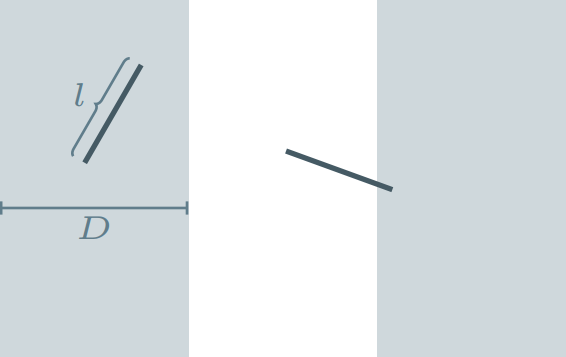
\includegraphics[width=\linewidth]{imagenes/buffon-1-1.png}
    \caption{Diagrama del experimento del buffon}
    \label{fig:buffon_exp}
\end{figure}

Teniendo en cuenta todo lo anterior y que ademas ambos parámetros son independientes (lo que asegura que $P(x,\theta)=P(x)P(\theta)$) podemos llegar a que la probabilidad de que toque esta dada por la ecuación \ref{eq:prob_buffon}

\begin{equation}
    P(t)=\int_{0}^{\pi}\int_{0}^{l/2sen\theta} \frac{2}{D}\frac{1}{\pi}dxd\theta=\frac{2l}{D\pi}
\label{eq:prob_buffon}
\end{equation}

Esto permite despejar a $\pi$ como $\pi= \frac{2l}{P(t)D}$, ahora para el experimento puedo tomar que $P(t)$ como la cantidad de agujas que tocan sobre la cantidad total de agujas tiradas ($N_{toque}/N_{total}$), donde usando la librería \textit{NumPy} de python se generan valores aleatorios que sigan las distribuciones uniformes de $x$ y de $\theta$. 

Para comprobar que tan buenas son las aproximaciones de $\pi$ con este experimento se realizaron 2 diagramas distintos, en el primero tiramos 10000 agujas y repetimos el experimento 100 mientras que en el segundo se fue aumentando la cantidad de agujas, en ambos se mantuvieron fijos el largo de la aguja y el ancho entre una linea y la otra.

\begin{figure}[h]
    \centering
    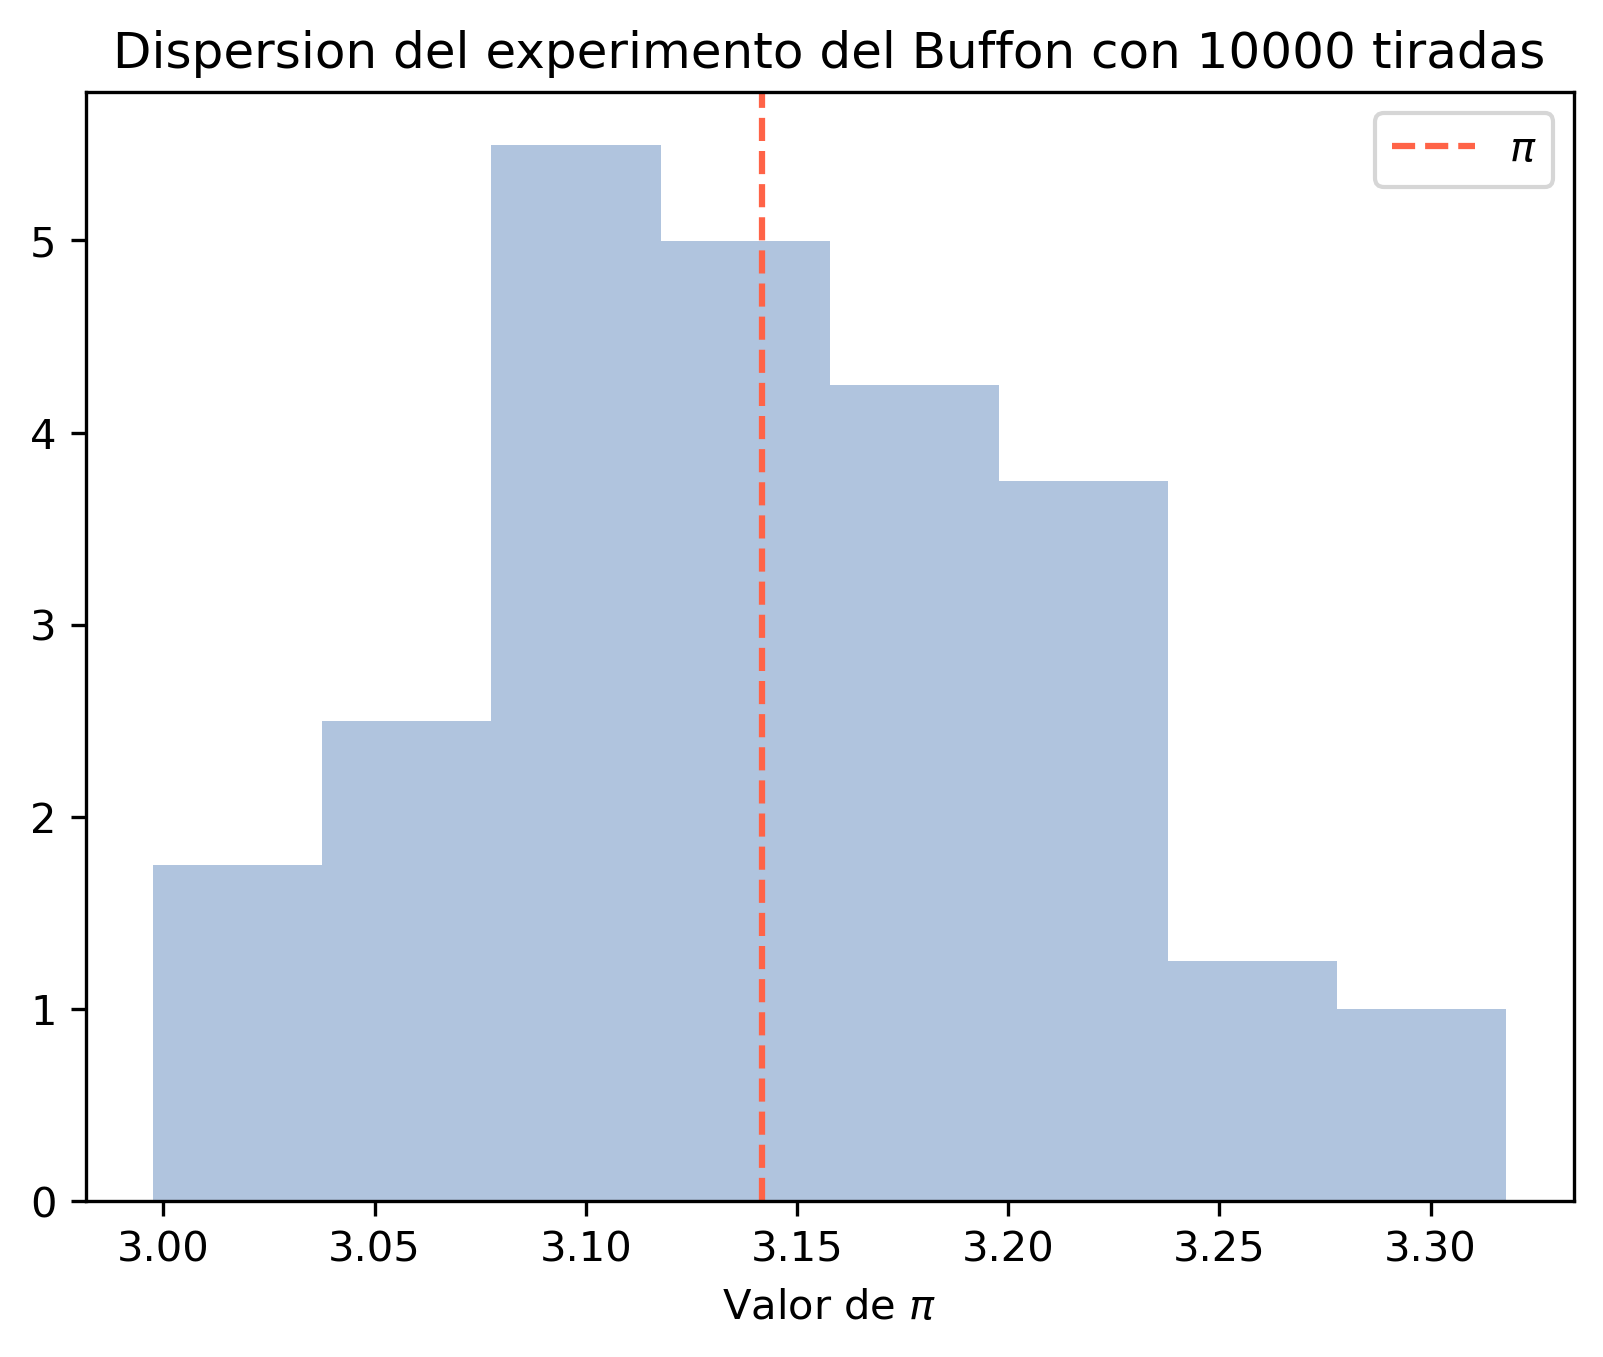
\includegraphics[width=\linewidth]{imagenes/buffon_x10000.png}
    \caption{Dispersión del valor de $\pi$ calculado con el experimento del buffon tirando 10000 agujas. En rojo el valor real de $\pi$}
    \label{fig:buffonx10000}
\end{figure}
\begin{figure}[h]
    \centering
    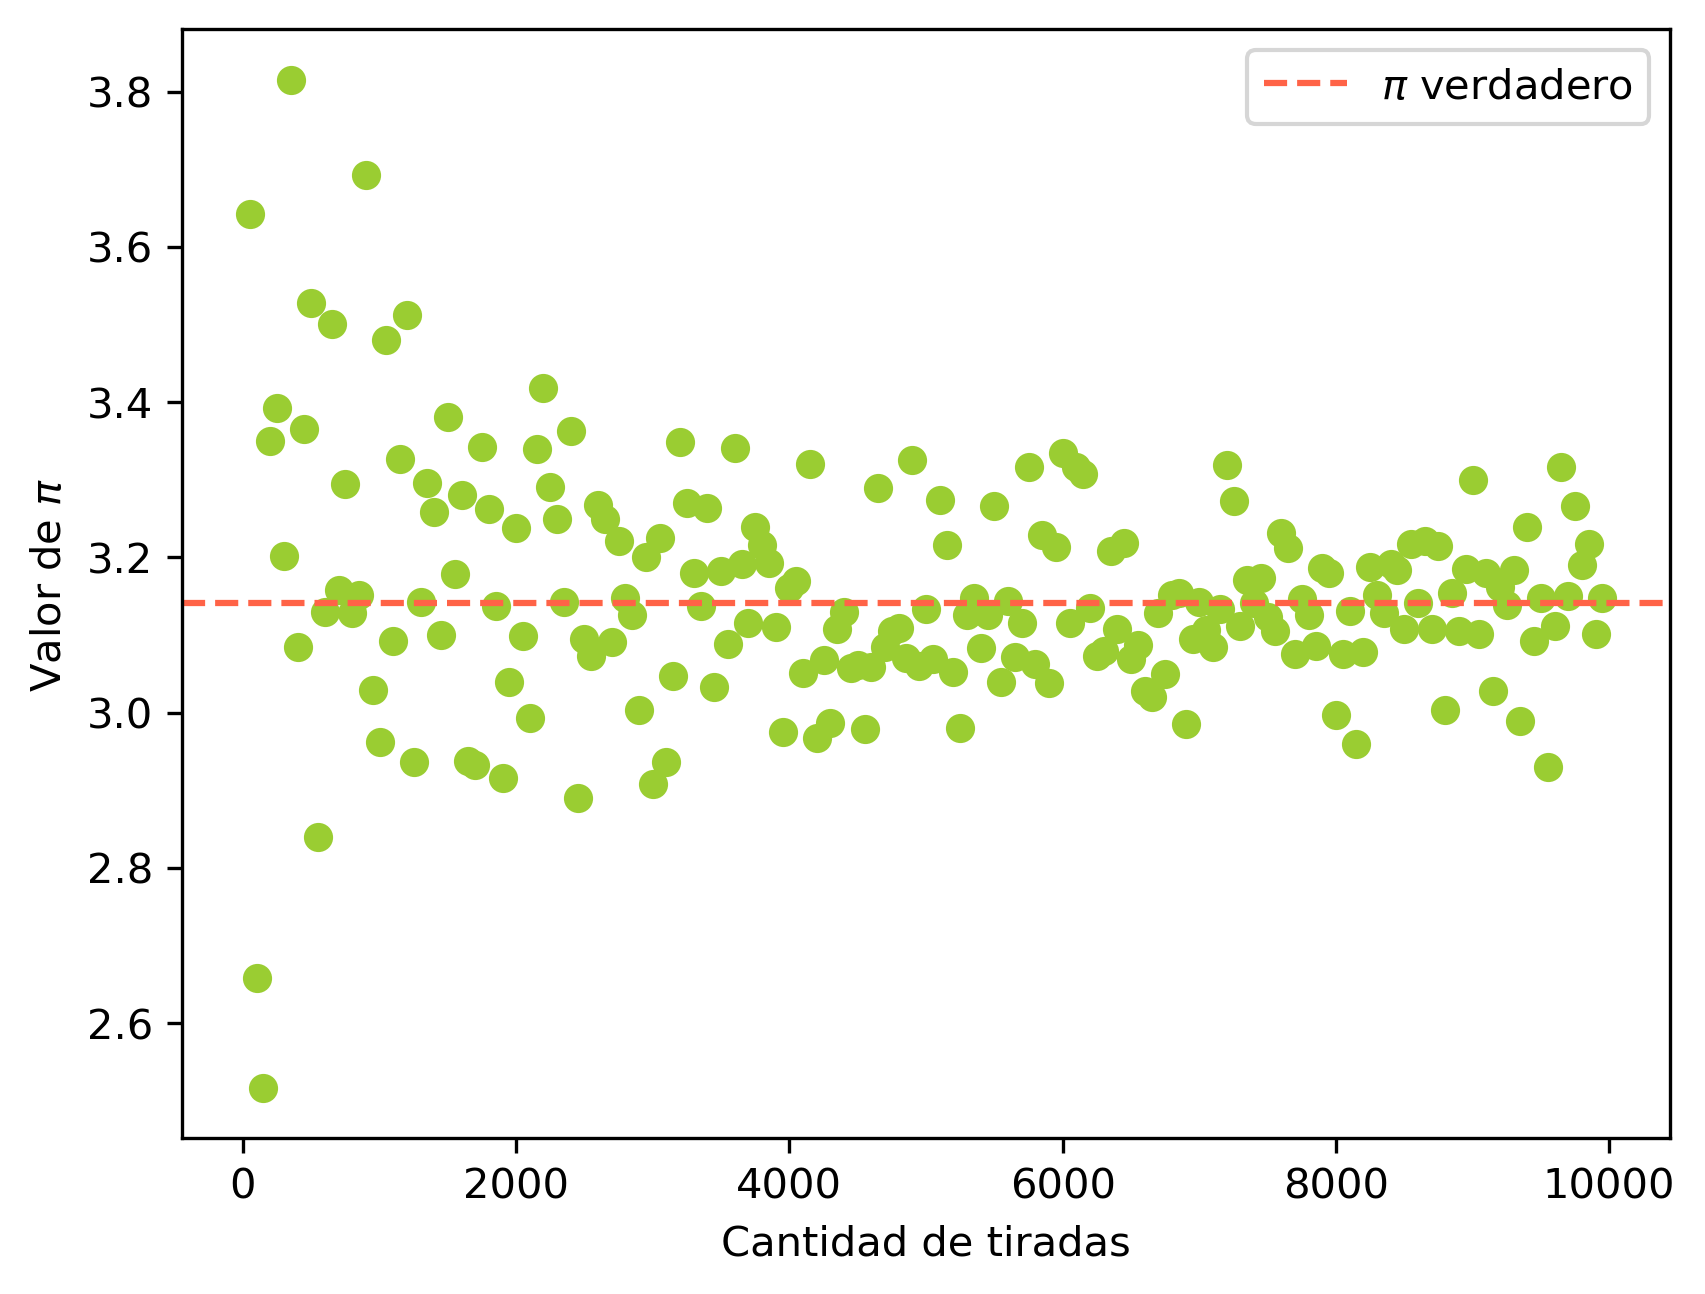
\includegraphics[width=\linewidth]{imagenes/buffon_conv.png}
    \caption{Valor medio de $\pi$ según la cantidad de agujas tiradas. En rojo el valor real de $\pi$.}
    \label{fig:buffonconv}
\end{figure}
\section{Conclusiones}
Se concluye que el método de la transformada inversa es un método que no presenta mayor complicación que encontrar la inversa de la función acumulada y que replica muy bien la distribución teórica sin grandes gastos computacionales. Todo lo contrario al experimento del buffon que requirió de una cantidad de datos muy grande para obtener un valor de $\pi$ con un error de $\pm0.08$, sin embargo resulta muy didáctico en términos de comprender como definir la probabilidad de un cierto resultado para un problema que en principio no esta relacionado con la probabilidad o la estadística.

La técnica de bootstrap también resulto muy efectiva, esto ya que computacionalmente se puede definir de manera general, de modo que cualquier parámetro que se desee conocer de la muestra general se pueda hacer reutilizando el código anterior. Algo que se destaca es que tanto las varianzas como las medias calculadas muestran la misma distribución, que en principio es independiente de la distribución original.   



\begin{figure*}
    \centering
    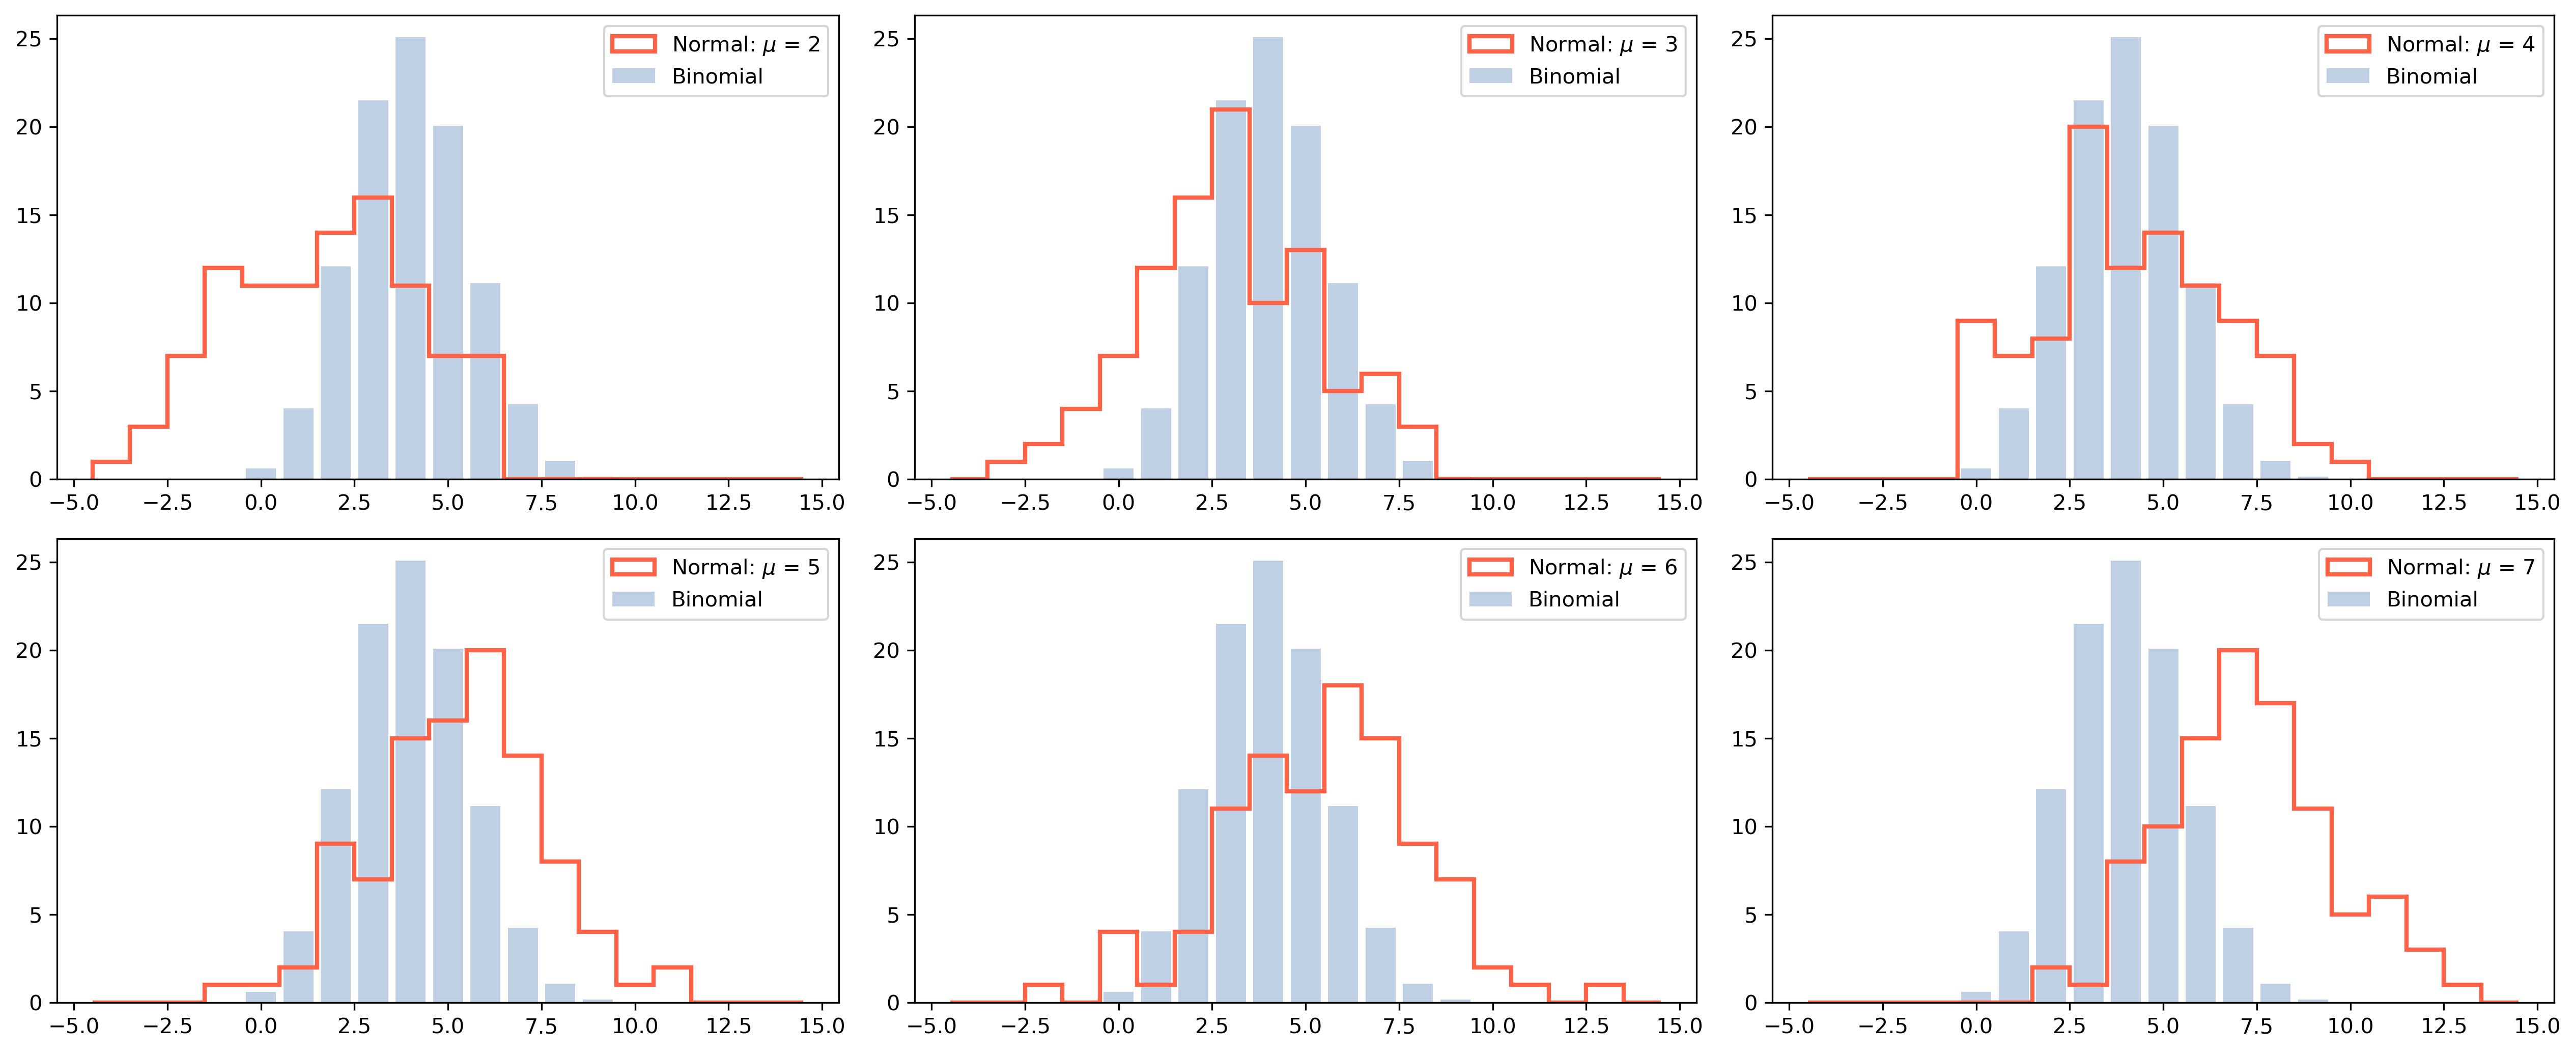
\includegraphics[width=\linewidth]{imagenes/binomial_vs_normal.png}
    \caption{Distribuciones de frecuencia de las variables aleatorias con distintos $\mu$ y superpuesto distribución binomial de interés}
    \label{fig:bin_vs_norm}
\end{figure*}
\bibliographystyle{baaa}
\small


\end{document}
